\documentclass{article}
\usepackage[a4paper, margin=1in]{geometry} % Adjust margins
\usepackage{graphicx} % Required for inserting images
\usepackage{subcaption}
\usepackage{hyperref}

\title{Search Algorithms and Markov Decision Processes \\ CS3IS7 Artificial Intelligence - Assignment 1}
\author{Conor Finlay | 20334367}
\date{1st March 2025}

\begin{document}

\maketitle

\section{Introduction}

\section{Maze Generation}

In this project, we generate mazes using the Recursive Backtracking algorithm. In the first instance, we generate what is called a "perfect maze", and then we create shortcuts through it to allow for multiple paths to be drawn between entrance and exit (and therefore the existence of "optimal" and "sub-optimal" paths). See \autoref{fig:mazes} for an illustration of these two types of mazes.

\subsection{Perfect Mazes}

The definition of a perfect maze is one where there is exactly \textit{one} path between any two points, where there are no loops, and there are no standalone walls (i.e. all walls must be connected to the borders of the maze). Here, we represent the maze as a 2d array, where \texttt{1}'s are walls and \texttt{0}'s are paths. We use the Recursive Backtracking algorithm to generate these mazes, as follows:

\begin{enumerate}
    \item The entire maze is initialised with walls (i.e. \texttt{1}'s)
    \item The algorithm begins at the starting position \texttt{(1, 1)}, marking it as a path
    \item It checks each direction (up, down, left, right) and, when it observes a wall \textbf{2 steps away}, it draws a path between the current point and that new point (i.e. joining them with a path). It then adds it to the stack, to be visited later.
    \item When the algorithm visits a cell with no wall neighbours, it "backtracks" and pops the cell off the stack.
    \item Once the stack is empty, all accessible cells have been visited.
\end{enumerate}

Since the algorithm only connects cells that are \textit{two blocks away}, where one of them is currently a wall, it never creates two paths between any two points.  This makes it a perfect maze. An example if this can be seen in \autoref{fig:perfectmaze}.

\subsection{Imperfect Mazes}

Once we have a perfect maze, we can turn it into an imperfect maze by removing some of the internal walls. Our algorithm identifies these walls, and turns a particular fraction of them into paths according to a provided parameter - \texttt{removal\_percentage}. This allows us to demonstrate how optimal the various algorithms are. In \autoref{fig:imperfectmaze}, you can see how an imperfect maze has multiple ways to get from entrance to exit.

\begin{figure}[h]
    \centering
    \begin{subfigure}[b]{0.45\textwidth}
        \centering
        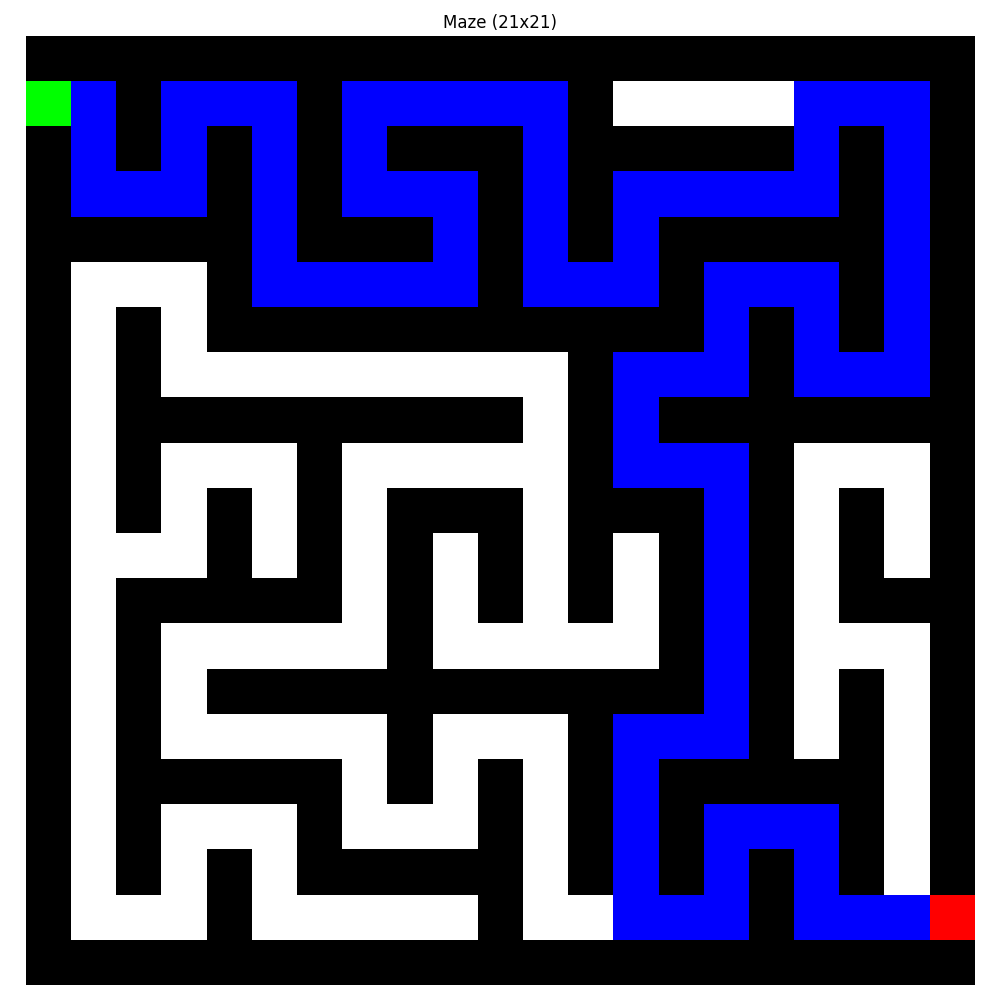
\includegraphics[width=\textwidth]{PerfectMaze.png}
        \caption{Perfect Maze}
        \label{fig:perfectmaze}
    \end{subfigure}
    \hfill
    \begin{subfigure}[b]{0.45\textwidth}
        \centering
        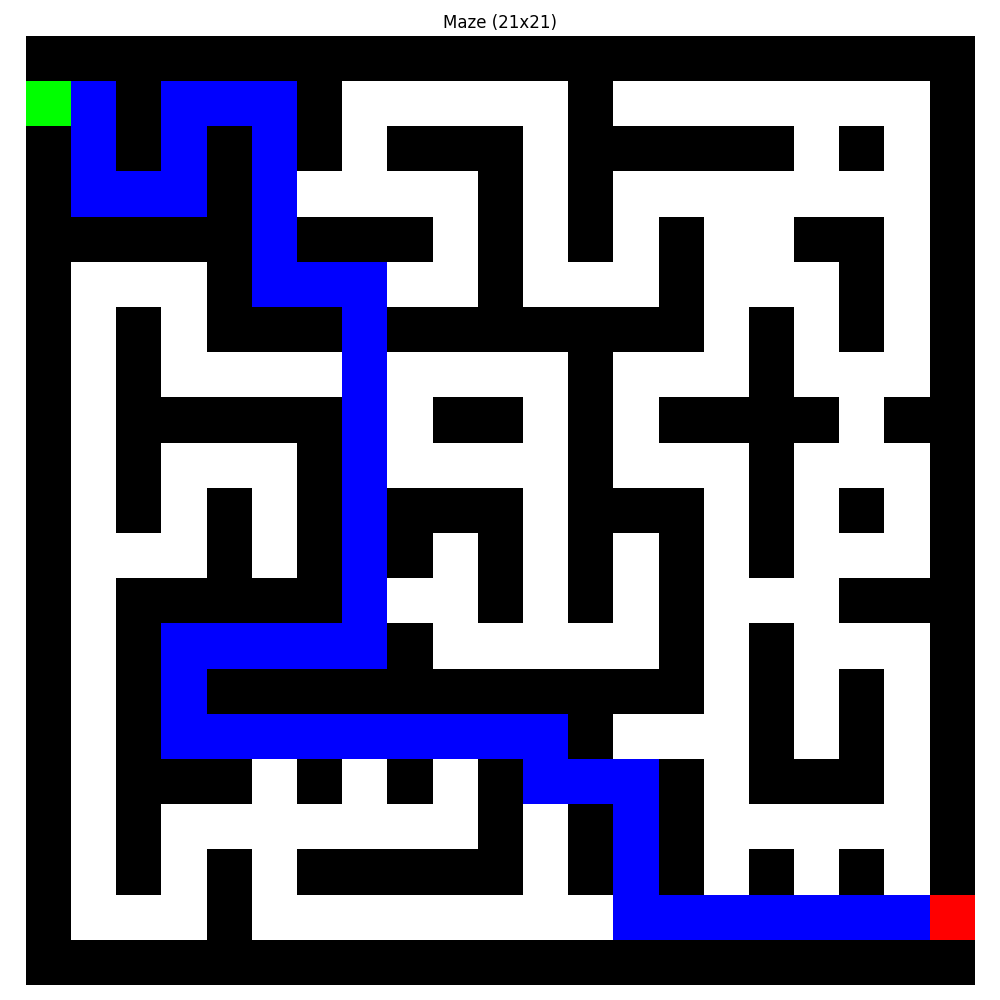
\includegraphics[width=\textwidth]{ImperfectMaze.png}
        \caption{Imperfect Maze}
        \label{fig:imperfectmaze}
    \end{subfigure}
    \caption{Perfect and Imperfect mazes with size (21x21)}
    \label{fig:mazes}
\end{figure}

\section{Search Algorithms}

In this section, we compare the performance of three path finding algorithms, namely, depth-first search (DFS), breadth-first search (BFS), and A*.  For the A* algorithm, we use the Manhattan distance from the current cell and the goal as a heuristic to guide the search. This choice is motivated in the second subsection, where we compare the performance of three different heuristics for the A* algorithm. But first, we'll examine the performance of the algorithms. 

\subsection{Comparison Between Search Algorithms}
\subsubsection{Perfect Maze}
We start by comparing the performance of the three algorithms on a perfect maze. We vary the maze sizes between (50x50) and (1000x1000), plotting the time taken for each of the algorithms to find the path as well as the number of nodes explored. The results can be seen in \autoref{fig:search_comparison}.

\begin{figure}[h]
    \centering
    \begin{subfigure}[b]{0.49\textwidth}
        \centering
        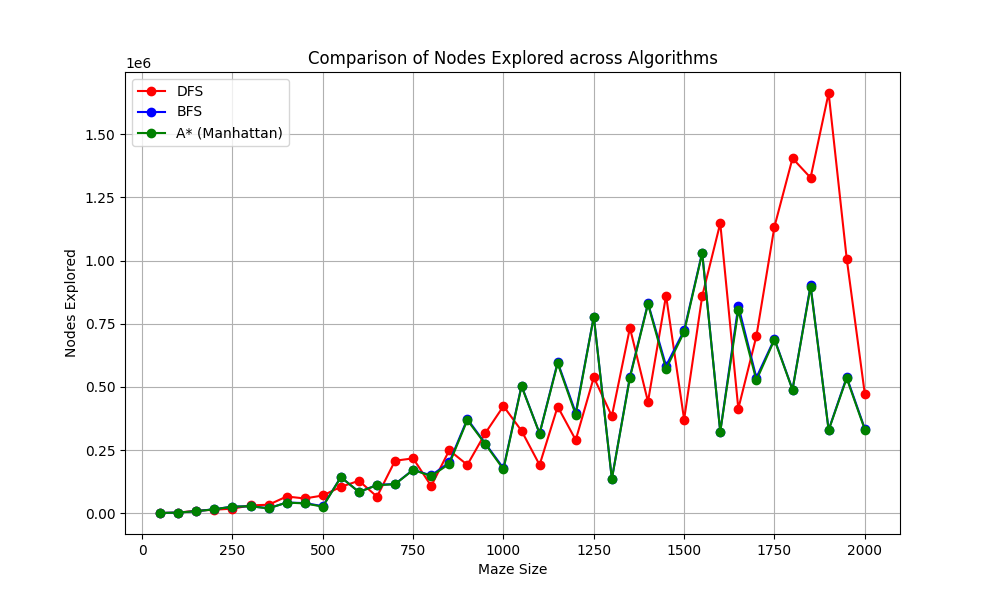
\includegraphics[width=\textwidth]{comparison_perfect_nodes_explored.png}
        \caption{Nodes Explored}
        \label{fig:nodes_explored_perfect_search}
    \end{subfigure}
    \begin{subfigure}[b]{0.49\textwidth}
        \centering
        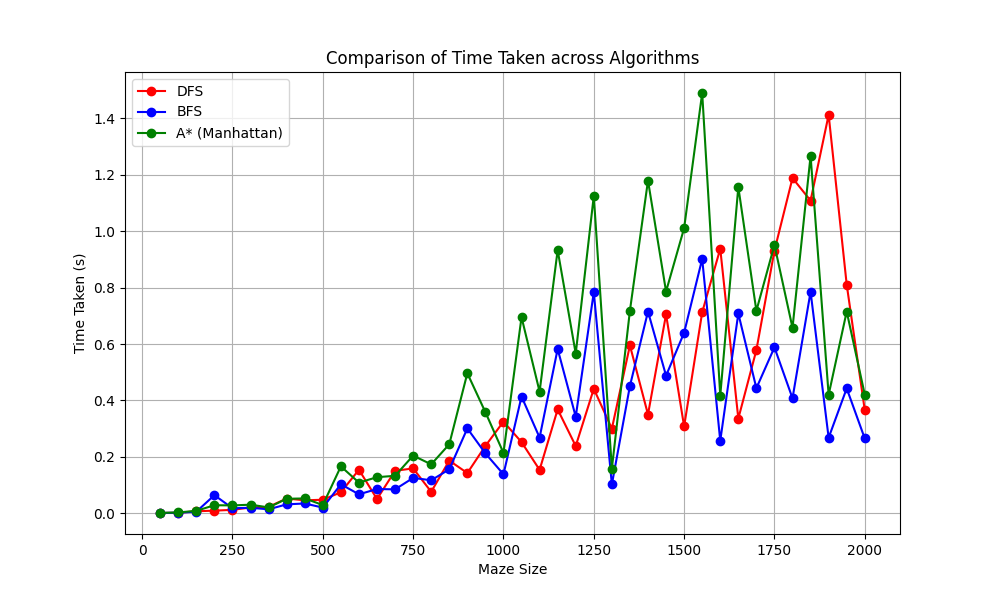
\includegraphics[width=\textwidth]{comparison_perfect_time_taken.png}
        \caption{Time Taken}
        \label{fig:time_taken_perfect_search}
    \end{subfigure}
    \caption{Performance Comparison of DFS, BFS, and A* for Different Perfect Maze Sizes}
    \label{fig:search_comparison}
\end{figure}

In \autoref{fig:nodes_explored_perfect_search}, we see that all algorithms explore a similar number of nodes. While we might expect DFS to explore fewer nodes, in these types of perfect mazes, the algorithms don't have much choice. We can see that for the last few very large mazes, DFS is more consistently "unlucky" in how it explores the maze. DFS and A* will not explore any paths longer than the path to the goal, where as DFS may get stuck exploring longer paths with dead ends before it finds the correct path to the goal.

It's clear from \autoref{fig:time_taken_perfect_search} that the time taken by each algorithm is a different story. The overall time taken by BFS and DFS almost perfectly match the number of nodes explored. A*, on the other hand, suffers from the additional overhead of calculating the heuristic. For a perfect maze, this heurstic is not particularly helpful and does not help A* to find the path any faster. There is not a strong reason to believe that, at any junction in the maze, the correct path is the one that heads in the direction of the goal. Additionally, since there is only one path to the goal, all algorithms are optimal. 

\begin{figure}[h]
    \centering
    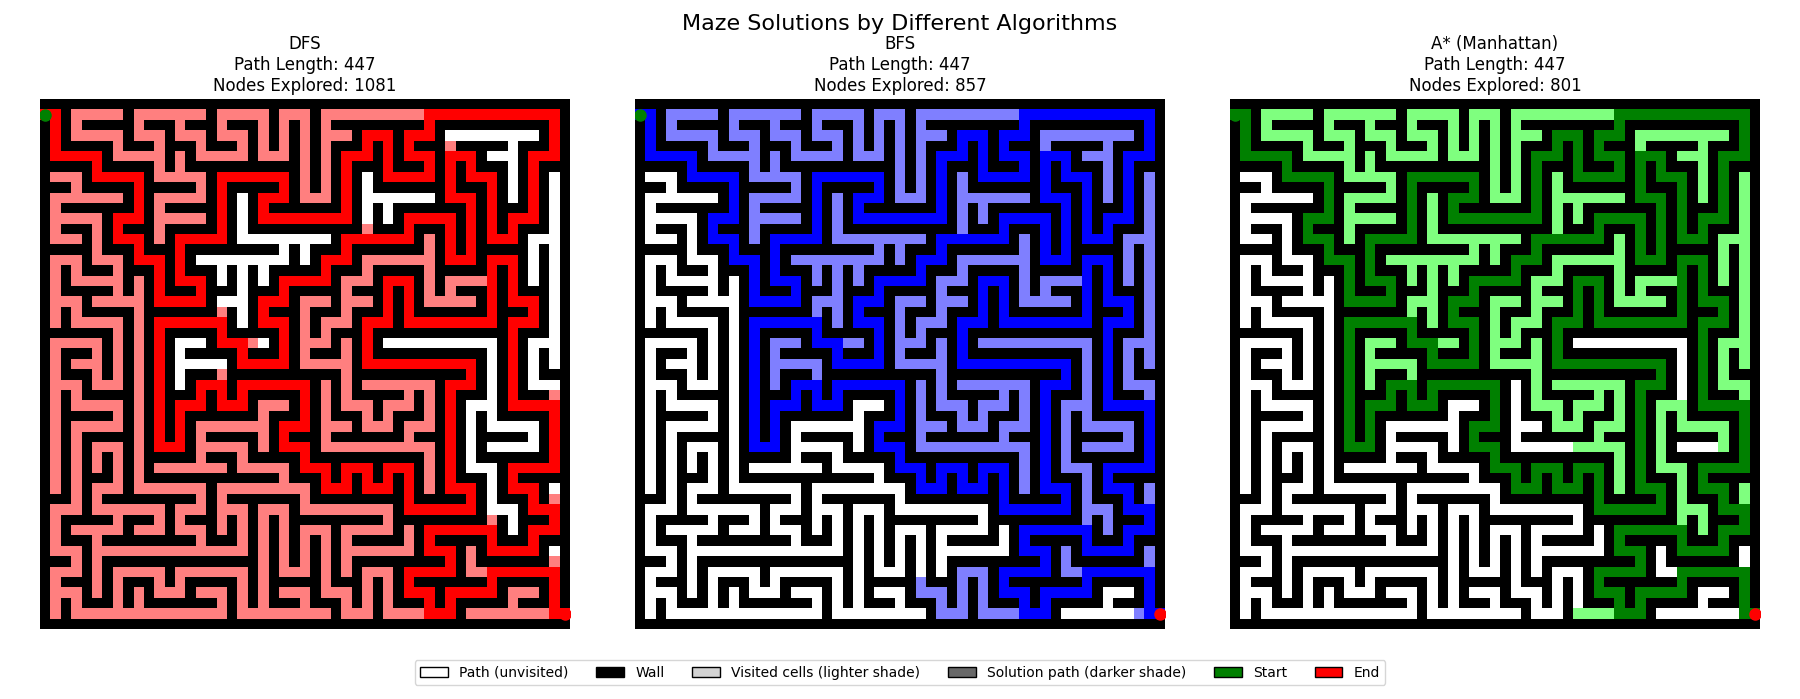
\includegraphics[width=\textwidth]{Solutions_perfectt.png}
    \caption{Solutions from DFS, BFS, and A* for a Perfect Maze}
    \label{fig:solutions_perfect}
\end{figure}

The behaviour of the algorithms is characterised by \autoref{fig:solutions_perfect}. We can see that DFS manages to avoid some of the dead ends explored by the other algorihms at first, but then takes a catestrophic wrong turn near the exit, causing it to explore many more nodes than the others. A* explores marginally fewer nodes than BFS, as it avoids going down paths that head away from the goal towards the end.

In \autoref{tab:astar_comparison}, we observe that A* takes roughly 1.75 times longer than DFS and 1.62 times longer than BFS to find the solution. Additionally, it seems to explore marginally more nodes than BFS, suggesting that the heuristic is holding the algorithm back on this type of maze.

\begin{table}[h]
    \centering
    \begin{tabular}{|l|c|c|}
        \hline
        \multicolumn{3}{|c|}{\textbf{Average Relative Performance (ratio of A* to other algorithms)}} \\
        \hline
        \textbf{Metric} & \textbf{A* / DFS ratio} & \textbf{A* / BFS ratio} \\
        \hline
        Nodes Explored & 1.0240 & 0.9816 \\
        \hline
        Time Taken & 1.7557 & 1.6262 \\
        \hline
    \end{tabular}
    \caption{Average relative performance of A* compared to other algorithms (perfect maze). Values represent the ratio of A* to the compared algorithm (values $> 1$ mean A* performs worse).}
    \label{tab:astar_comparison}
\end{table}

\subsubsection{Imperfect Maze}

In order to observe the differences between the algorithms in terms of optimality (finding the shortest path) and efficiency (in terms of nodes explored), we test them on an \textit{imperfect} maze. We remove 10\% of the walls from a perfect maze, and then test the algorithms on the resulting maze. The results can seen in \autoref{fig:search_comparison_imperfect}.

\begin{figure}[h]
    \centering
    \begin{subfigure}[b]{0.49\textwidth}
        \centering
        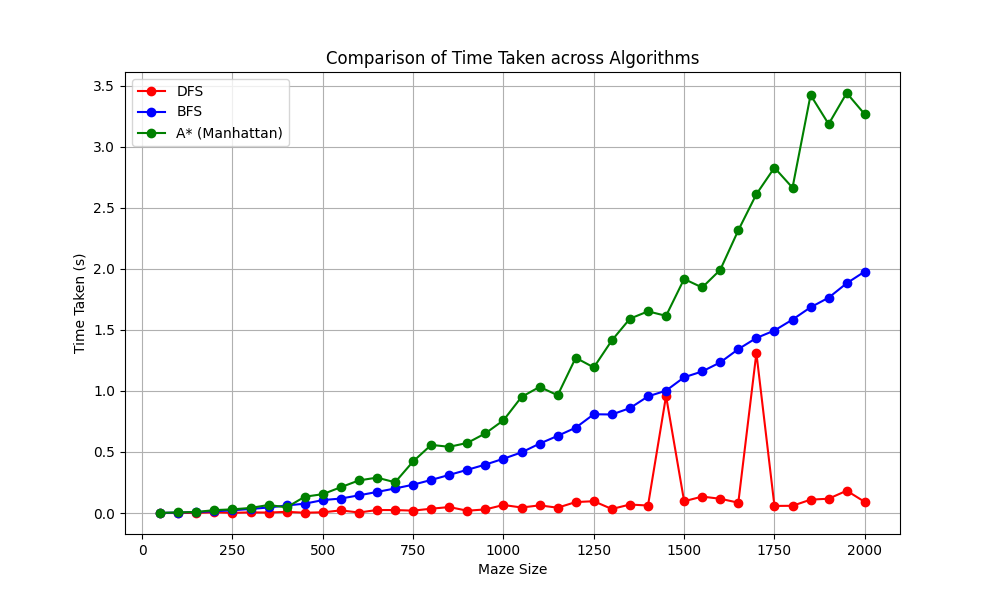
\includegraphics[width=\textwidth]{Time Taken imperfect.png}
        \caption{Time Taken}
        \label{fig:time_taken_imperfect_search}
    \end{subfigure}
    \begin{subfigure}[b]{0.49\textwidth}
        \centering
        \includegraphics[width=\textwidth]{Nodes Explored imperfect.png}
        \caption{Nodes Explored}
        \label{fig:nodes_explored_imperfect_search}
    \end{subfigure}
    \caption{Performance Comparison of DFS, BFS, and A* for Different Imperfect Maze Sizes}
    \label{fig:search_comparison_imperfect}
\end{figure}

Looking at \autoref{fig:time_taken_imperfect_search}, we see that A* takes the longest out of all of the algorithms, nudging ahead of BFS. This is now more in line with the expected complexity of these algorithms - BFS shows a broadly linear time complexity ($O(n)$) while A* is more like $O(n \log n)$ due to the max heap it maintains for selecting the next node to explore. The time taken for DFS to find a solution is now much quicker, as it benefits from finding \textit{any} path to the goal.

If we now consider the number of nodes explored, as well as the optimality of the path found, the results are somewhat flipped on their head. First, considering path length, BFS and A* are both \textit{optimal}, and will always find the shortest path to the goal. This is not true for DFS. On average, across all maze sizes tested, the path length found by DFS was on average \textbf{12.05 times longer} than the optimal paths found by BFS and A*.

If we turn to the number of nodes expored, DFS naturally explores the least. However, among the optimal algorithms, A* explores fewer nodes than BFS, guided by the heuristic which is now more helpful given the altered structure of the maze. These results are summarised in \autoref{tab:astar_comparison_imperfect} and illustrated in \autoref{fig:solutions_imperfect}.
\begin{table}[h]
    \centering
    \begin{tabular}{|l|c|c|}
        \hline
        \multicolumn{3}{|c|}{\textbf{Average Relative Performance (ratio of A* to other algorithms)}} \\
        \hline
        \textbf{Metric} & \textbf{A* / DFS ratio} & \textbf{A* / BFS ratio} \\
        \hline
        Nodes Explored & 9.2184 & 0.7768 \\
        \hline
        Time Taken & 21.0405 & 1.6368 \\
        \hline
    \end{tabular}
    \caption{Average relative performance of A* compared to other algorithms (imperfect maze). Values represent the ratio of A* to the compared algorithm (values $> 1$ mean A* performs worse).}
    \label{tab:astar_comparison_imperfect}
\end{table}

\begin{figure}[h]
    \centering
    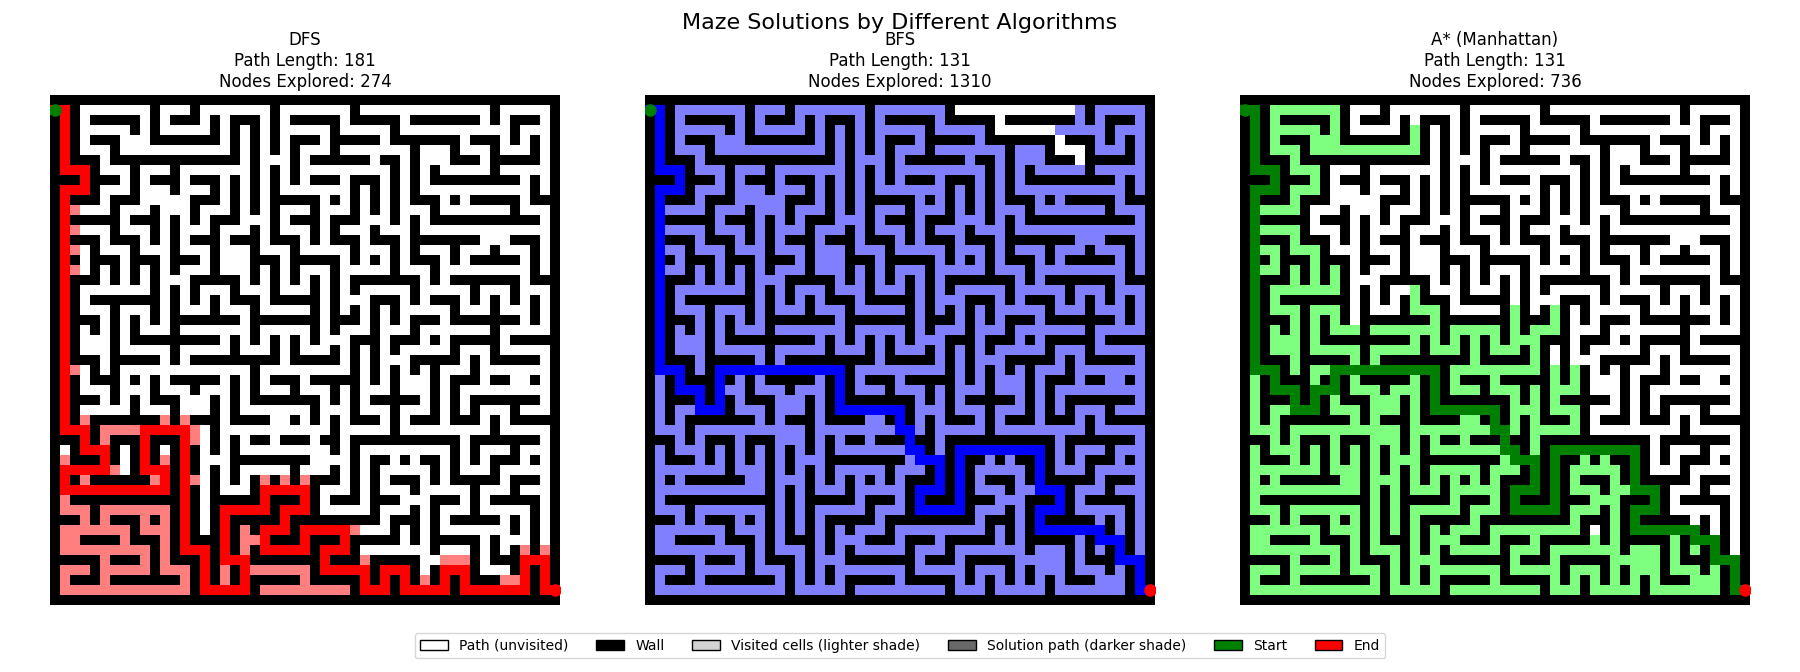
\includegraphics[width=\textwidth]{imperfect maze solutions search.png}
    \caption{Solutions from DFS, BFS, and A* for an Imperfect Maze}
    \label{fig:solutions_imperfect}
\end{figure}

\subsection{Comparison of A* Heuristics}

In this section, we motivate the use of the Manhattan distance as a heuristic for the A* algorithm. To do this, we compare the performance of A* using the Manhattan distance, Euclidean distance, and Chebyshev distance. These heuristics are defined as follows:
\vspace{1em}

\textbf{Manhattan distance: } 
$$h(n) = |x_n - x_{goal}| + |y_n - y_{goal}|$$

\textbf{Euclidean distance: } 
$$h(n) = \sqrt{(x_n - x_{goal})^2 + (y_n - y_{goal})^2}$$

\textbf{Chebyshev distance: } 
$$h(n) = \max(|x_n - x_{goal}|, |y_n - y_{goal}|)$$

When tested on imperfect mazes of sizes between 50 and 1000 like in the previous section, the manhattan distance heuristic consistently outperformed the other two. The results are summarised in \autoref{tab:heuristic_comparison}.

\begin{table}[h]
    \centering
    \begin{tabular}{|l|c|c|}
        \hline
        \multicolumn{3}{|c|}{\textbf{Average Relative Performance (ratio to Manhattan)}} \\
        \hline
        \textbf{Metric} & \textbf{A* (Euclidean)} & \textbf{A* (Diagonal)} \\
        \hline
        Nodes Explored & 1.1818 & 1.2136 \\
        \hline
        Time Taken & 1.1759 & 1.2293 \\
        \hline
    \end{tabular}
    \caption{Comparison of different heuristics for A* algorithm on imperfect mazes. Values represent the ratio to Manhattan distance (values $> 1$ mean Manhattan performs better).}
    \label{tab:heuristic_comparison}
\end{table}

\section{Markov Decision Processes}
In this section, we compare the performance of two different algorithms for solving MDPs, namely, policy iteration and value iteration. 

\subsection{Implementation Details}
When interpreting this problem as a Markov Decision Process, we define the state space as all of the accessible cells in the maze. The action space is the set of up, down, left, and right movements. The only reward function required is the reward for exiting the maze, which we set to 100.0. A discount factor of 0.99 encourages the agent to find the shortest path to the exit.

Initially, we had used a negative reward for each step taken to encourage the agent to find the shortest path to the exit. However, since there are no other factors at play in this problem (i.e. no other rewards, no probabilistic movement, etc.), the discount factor alone is enough to encourage the agent to find the shortest path to the exit.

For Value Iteration, our convergence criterion is $\epsilon = 0.001$, meaning that we continue iterating until the maximum change in utility between iterations is less than 0.001.
For Policy Iteration, we simply continue until the policy does not change between runs. However, for the policy evaluation step, we continue iterating until that same convergence criterion is met.
\subsection{Policy Iteration vs. Value Iteration}

To compare the performance of the two algorithms, we test them on a range of imperfect maze sizes from (25x25) to (150x150) in increments of 25. The results can be seen in \autoref{fig:policy_iteration_vs_value_iteration}.

\begin{figure}[h]
    \centering
    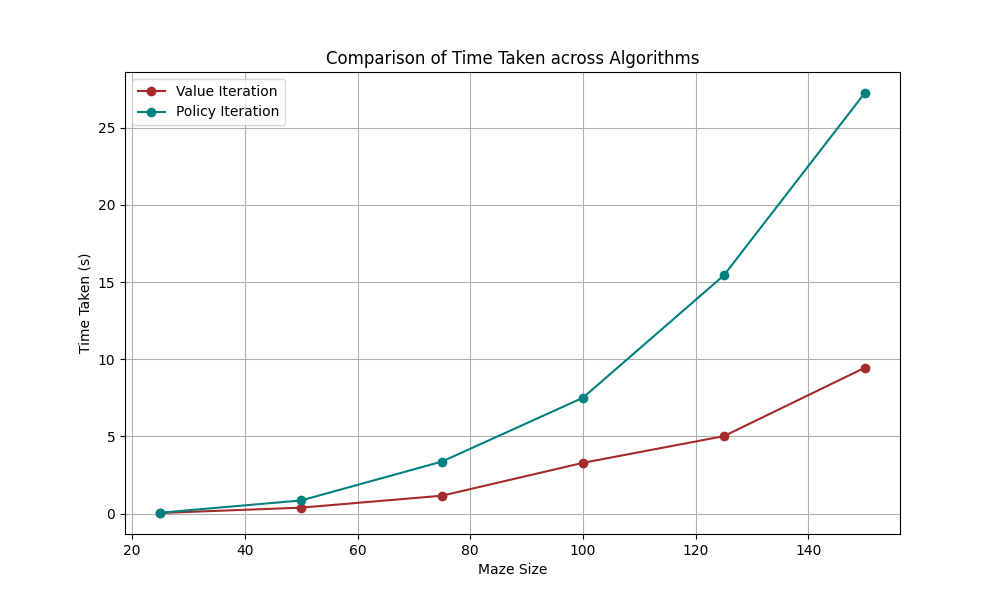
\includegraphics[width=\textwidth]{Value iteration vs. policy time .png}
    \caption{Comparison of Policy Iteration and Value Iteration}
    \label{fig:policy_iteration_vs_value_iteration}
\end{figure}

Policy iteration is clearly slower than value iteration thanks to its expensive policy evaluation step. Although it may have stronger convergence guarantees in general, for the simple case of a maze, value iteration is a more appropriate solution.

It's also very clear that these algorithms take far longer than the search algorithms to find a solution. Indeed, the do always find the optimal solution, but they explore all possible states and perform many updates to do this. We discuss this in the next section.

\section{Search Algorithms vs. MDPs}

\autoref{fig:all_algos_time} shows the disparity in time taken between the search algorithms and the MDP algorithms. The MDP algorithms are incredibly inefficient for this problem, and there is no reason to use them here without the following additions:

\begin{itemize}
    \item \textbf{Other rewards:} If there were other rewards in the maze (e.g. diamonds to find, or pits to avoid), the MDP algorithms would be uniquely suited to solve this problem in a way that search algorithms cannot.
    \item \textbf{Probabilistic movement:} If the agent was inclined to move with some randomness (e.g. when wanting to move forward, you move left with some probability), the MDP algorithms would be able to plan based on this information.
\end{itemize}

\begin{figure}[h]
    \centering
    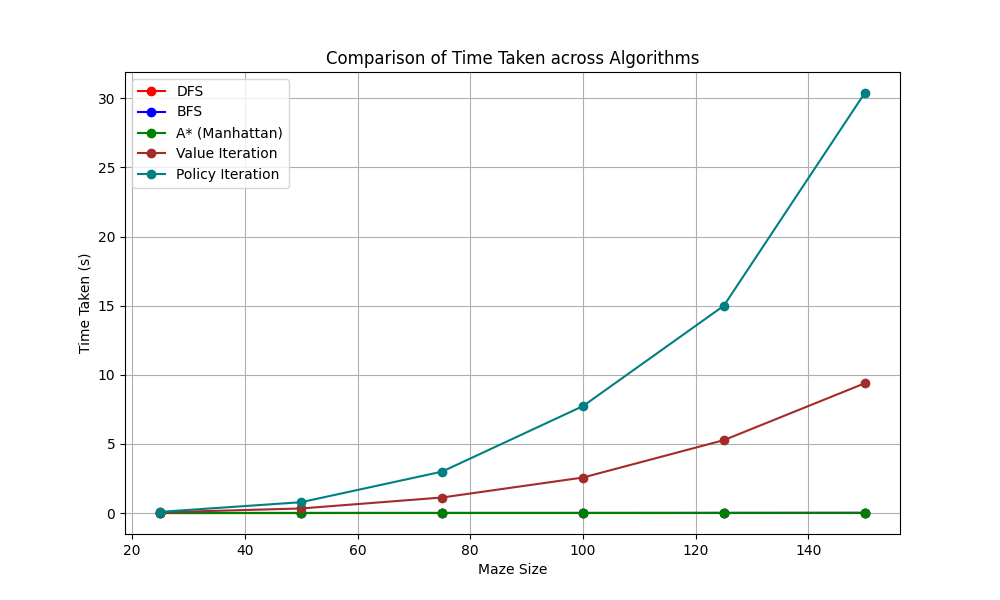
\includegraphics[width=\textwidth]{all algos time.png}
    \caption{Comparison of all algorithms}
    \label{fig:all_algos_time}
\end{figure}

However, in the absence of these features, there really is no reason to use MDPs here. The search algorithms have demonstrated that they are the best approach performing straight forward pathfinding, which is exactly what we have here.




\end{document}
